% !TEX root = ../main.tex
\section{Ứng dụng: hệ thống bãi giữ xe mô phỏng}\label{sec:app}

Để đưa mô hình vào một tình huống sử dụng cụ thể, dự án xây dựng một bãi giữ xe mô phỏng 3D chạy trên trình duyệt, nối với mô hình nhận diện thật qua REST API. Người dùng đóng vai người gửi xe, bảo vệ và camera ở cổng.

\begin{figure}[H]
\centering
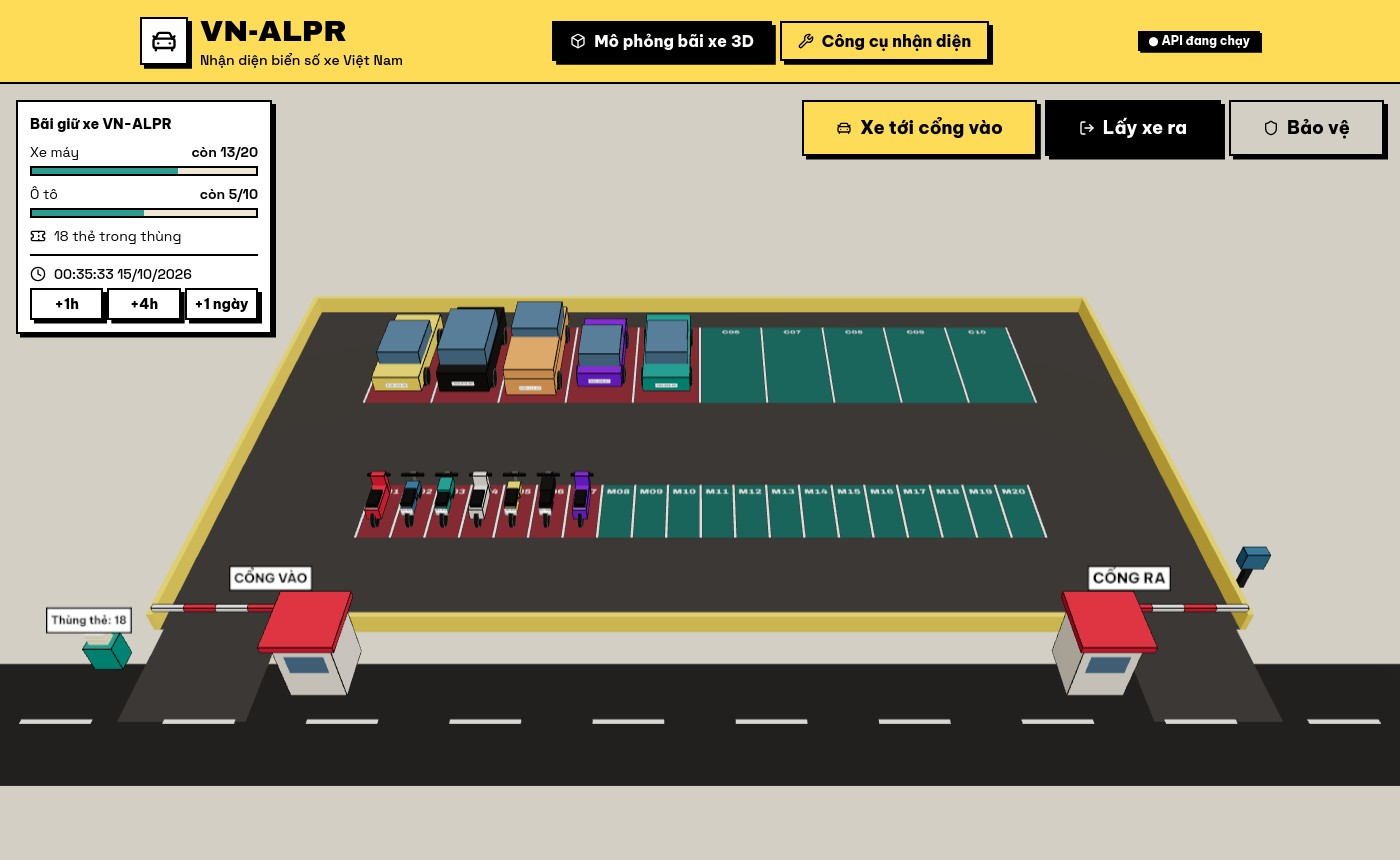
\includegraphics[width=\linewidth]{figures/sim_overview.jpg}
\caption{Bãi giữ xe mô phỏng: 20 chỗ xe máy, 10 chỗ ô tô (ô đỏ là ô có xe), cổng vào với thùng thẻ ở bên trái, cổng ra với đầu đọc thẻ ở bên phải. Khung bên trái cho biết số chỗ trống, số thẻ trong thùng và đồng hồ mô phỏng.}
\label{fig:sim-overview}
\end{figure}

\subsection{Luồng nghiệp vụ}
\paragraph{Xe vào.} Người dùng chọn loại xe, kiểu dáng và màu (4 kiểu ô tô, 3 kiểu xe máy, 9 màu), xe chạy tới cổng vào. Ảnh biển số được tải lên hoặc chụp bằng webcam. Mô hình đọc biển, và người gửi \emph{được sửa tay} nếu mô hình đọc sai; ô nhập kiểm tra định dạng biển ngay khi gõ bằng chính hàm hậu xử lý của pipeline. Sau đó người gửi bấm vào thùng thẻ để lấy thẻ, xác nhận, barrier mở và xe chạy vào ô đỗ được cấp (Hình~\ref{fig:sim-entry}).

\paragraph{Xe ra.} Người dùng chọn xe trong bãi, xe chạy ra cổng ra. Khách đưa thẻ (hoặc báo mất thẻ), camera chụp biển số, và hệ thống so biển đọc được với biển đã gắn với thẻ lúc vào (Hình~\ref{fig:sim-exit}). Biển số lúc ra \emph{không} cho người lái sửa tay: nếu được sửa, ai cầm thẻ cũng có thể gõ đúng biển để lấy xe. Khi kết quả không khớp, chỉ bảo vệ được duyệt cho xe ra và bắt buộc phải ghi lý do.

\begin{figure}[H]
\centering
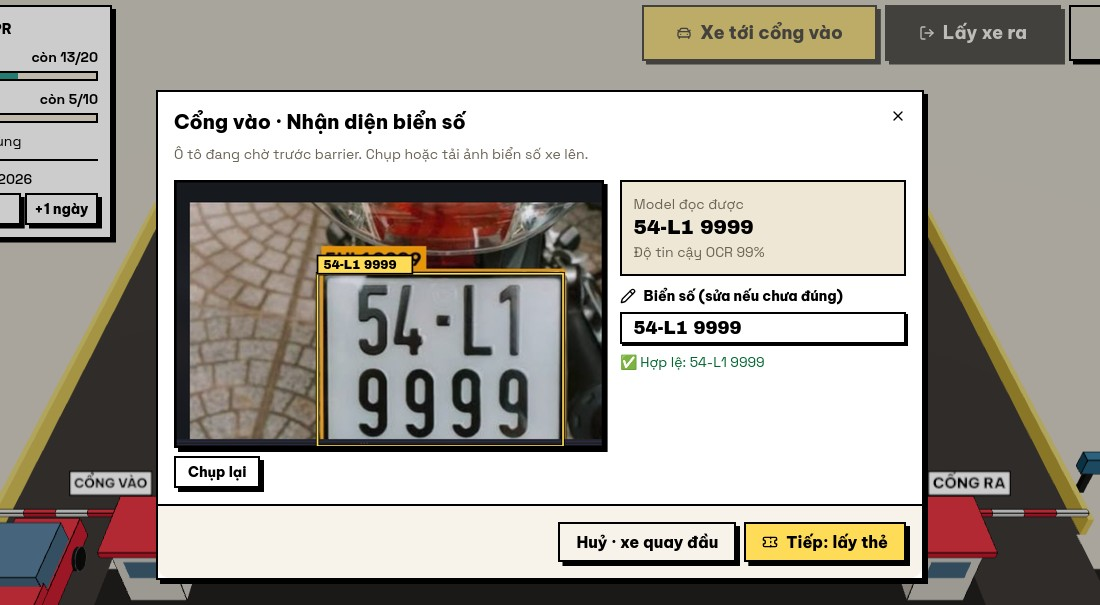
\includegraphics[width=0.92\linewidth]{figures/sim_entry.jpg}
\caption{Cổng vào: mô hình đọc biển \code{54-L1 9999} với độ tin cậy 98\,\%, người gửi có thể sửa trước khi lấy thẻ.}
\label{fig:sim-entry}
\end{figure}

\begin{figure}[H]
\centering
\begin{subfigure}[b]{0.66\linewidth}
  \centering
  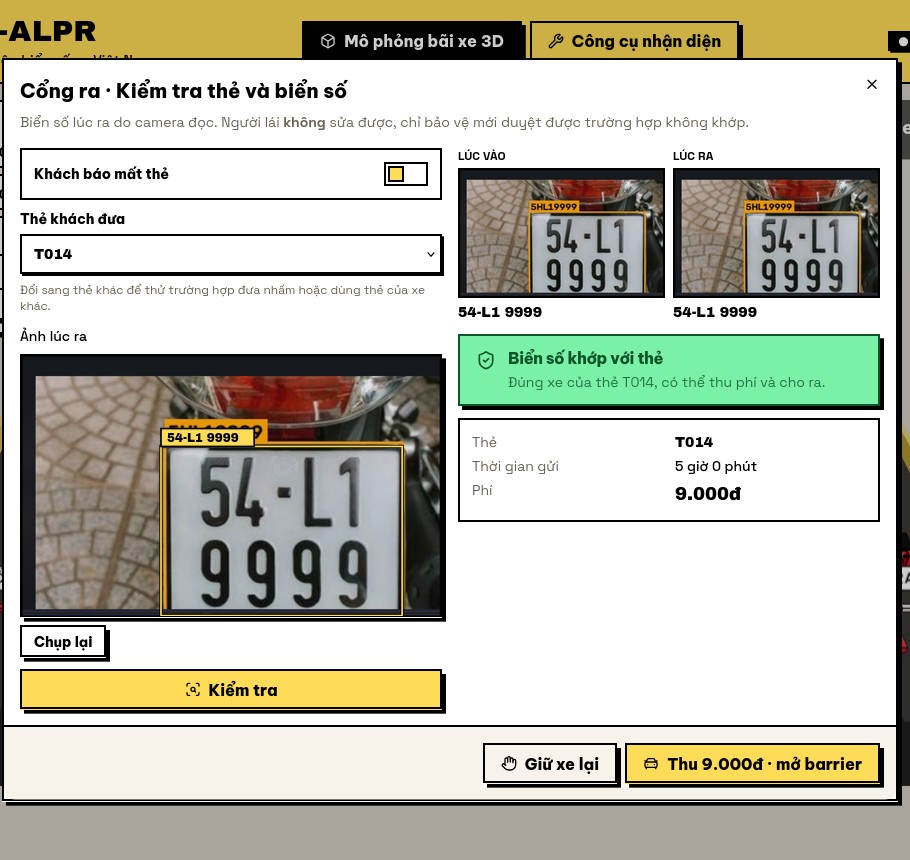
\includegraphics[width=\linewidth]{figures/sim_exit.jpg}
  \caption{Cổng ra: ảnh lúc vào và lúc ra, kết quả so khớp, thời gian gửi và phí.}
  \label{fig:sim-exit}
\end{subfigure}\hfill
\begin{subfigure}[b]{0.31\linewidth}
  \centering
  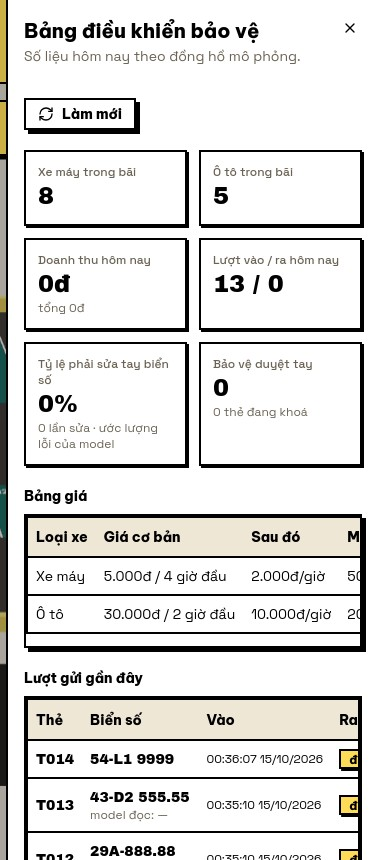
\includegraphics[width=\linewidth]{figures/sim_dashboard.jpg}
  \caption{Bảng điều khiển bảo vệ.}
  \label{fig:sim-dashboard}
\end{subfigure}
\caption{Màn hình ở cổng ra và của bảo vệ.}
\end{figure}

\subsection{Luật nghiệp vụ}
\begin{itemize}[nosep]
  \item \textbf{Thẻ và chỗ đỗ.} Bãi có 30 thẻ và 30 ô (20 xe máy, 10 ô tô). Thẻ được phát theo thứ tự ``trả về lâu nhất ra trước''. Hệ thống từ chối khi hết chỗ cho loại xe đó, khi thẻ không còn trong thùng, hoặc khi biển số đã có trong bãi (chặn gửi trùng).
  \item \textbf{Phí.} Mỗi loại xe có một bảng giá: giá cơ bản cho $h_0$ giờ đầu, sau đó $p$ đồng cho \emph{mỗi giờ đã bắt đầu}:
  \begin{equation}
    \text{phí} = b + p \cdot \max\!\left(0,\ \left\lceil t - h_0 \right\rceil\right) + \mathbb{1}[\text{mất thẻ}] \cdot \ell,
  \end{equation}
  với $t$ là số giờ gửi. Xe máy: $b = 5\,000$đ, $h_0 = 4$, $p = 2\,000$đ, $\ell = 50\,000$đ. Ô tô: $b = 30\,000$đ, $h_0 = 2$, $p = 10\,000$đ, $\ell = 200\,000$đ. Toàn bộ nằm trong \code{configs/parking.yaml}.
  \item \textbf{So khớp ở cổng ra.} Gọi $d$ là khoảng cách Levenshtein giữa biển trên thẻ và biển đọc được gần nhất trong ảnh, $c$ là độ tin cậy OCR. Kết quả là \emph{khớp} nếu $d = 0$; \emph{nghi đọc sai} nếu $d \le 1$ và $c < 0{,}95$ (hoặc không đọc được biển nào); còn lại là \emph{không khớp}. Mức ``nghi đọc sai'' giúp bảo vệ phân biệt lỗi của mô hình với một chiếc xe khác.
  \item \textbf{Thẻ của xe khác.} Nếu thẻ đưa ra gắn với một xe khác trong bãi, hệ thống báo và không cho ra.
  \item \textbf{Mất thẻ.} Bảo vệ tra cứu theo biển số, thu thêm phí mất thẻ và \emph{khoá} thẻ cũ để thẻ đó không mở được cổng nữa; thẻ chỉ về thùng khi bảo vệ xác nhận đã tìm thấy.
\end{itemize}

\paragraph{Vòng phản hồi dữ liệu.} Mỗi lần người gửi sửa tay biển số ở cổng vào, hệ thống có thêm một cặp (ảnh, biển đúng). Tỉ lệ phải sửa tay được hiển thị trên bảng điều khiển như một ước lượng độ chính xác của mô hình ngoài thực tế, và các cặp này xuất được thành tập dữ liệu dòng chữ (\code{labels.tsv}) để fine-tune CRNN.

\paragraph{Đồng hồ mô phỏng.} Để trình diễn cách tính phí mà không phải chờ, đồng hồ của bãi có thể tua nhanh (+1 giờ, +4 giờ, +1 ngày). Tính năng này chỉ dùng cho demo và tắt được trong cấu hình.

\subsection{Giao diện}
Giao diện viết bằng React, Vite và Tailwind CSS, theo phong cách \emph{neobrutalism} (viền đen dày, bóng đổ cứng). Cảnh 3D dựng bằng React Three Fiber; xe là mô hình low-poly dựng từ khối hộp và trụ, biển số được vẽ lên texture từ chuỗi đã xác nhận. Một máy trạng thái duy nhất (thư viện zustand) điều khiển cả hoạt cảnh lẫn hộp thoại, để hai phần này không bao giờ lệch nhau:
\begin{center}
\footnotesize
\begin{tabular}{rl}
Vào: & chọn xe $\to$ tới cổng $\to$ nhận diện $\to$ lấy thẻ $\to$ xác nhận $\to$ vào ô đỗ \\
Ra: & chọn xe $\to$ tới cổng $\to$ kiểm tra $\to$ ra khỏi bãi (hoặc giữ lại $\to$ về ô đỗ)
\end{tabular}
\end{center}

\subsection{Kiến trúc backend}
Backend (FastAPI) tổ chức theo kiến trúc phân lớp (Hình~\ref{fig:layers}). Phụ thuộc chỉ đi một chiều: tầng API gọi tầng dịch vụ, tầng dịch vụ dùng luật của tầng miền và các giao diện mà tầng hạ tầng cài đặt. Thư viện học máy \code{src/alpr} tách hẳn khỏi ứng dụng.

\begin{figure}[H]
\centering
\resizebox{\linewidth}{!}{%
\begin{tikzpicture}[
  layer/.style={draw, rounded corners, minimum height=0.95cm, text width=12.2cm, align=left, font=\small, inner sep=5pt},
  arr/.style={-{Stealth[length=2mm]}, thick}
]
\node[layer, fill=yellow!25] (api) {\textbf{api}: router, schema Pydantic cho request và response, một bộ chuyển lỗi nghiệp vụ thành mã HTTP};
\node[layer, fill=blue!8, below=0.35cm of api] (svc) {\textbf{services}: \code{ParkingService}, \code{GateLog}, \code{RecognitionService}, xuất dữ liệu huấn luyện};
\node[layer, fill=green!10, below=0.35cm of svc, text width=5.8cm, xshift=-3.2cm] (dom) {\textbf{domain}: thực thể và luật thuần (tính phí, so khớp biển), không SQL hay HTTP};
\node[layer, fill=red!8, right=0.3cm of dom, text width=5.8cm] (infra) {\textbf{infra}: SQLite + migration, repository, kho ảnh, đồng hồ};
\draw[arr] (api) -- (svc);
\draw[arr] (svc.south -| dom.north) -- (dom.north);
\draw[arr] (svc.south -| infra.north) -- (infra.north);
\end{tikzpicture}}
\caption{Các tầng của backend. Một mô-đun ``composition root'' duy nhất lắp các tầng lại với nhau.}
\label{fig:layers}
\end{figure}

Một số quyết định đáng chú ý:
\begin{itemize}[nosep]
  \item \textbf{Giao dịch (transaction).} Ghi một lượt gửi xe, đổi trạng thái thẻ và ghi nhật ký cổng nằm trong cùng một giao dịch; khi một luật từ chối giữa chừng, không còn dữ liệu dở dang.
  \item \textbf{Migration có phiên bản.} Lược đồ cơ sở dữ liệu là các tệp SQL đánh số; \code{PRAGMA user\_version} ghi lại tệp cuối đã áp dụng, nên cơ sở dữ liệu cũ tự được nâng cấp mà không mất dữ liệu.
  \item \textbf{Đồng hồ là một phụ thuộc.} Dịch vụ hỏi giờ qua giao diện \code{Clock}: thời gian thực khi chạy, đồng hồ cố định trong kiểm thử, đồng hồ tua được trong demo.
  \item \textbf{Kiểm thử.} 84 bài kiểm thử tự động (pytest) chạy không cần trọng số mô hình, nhờ pipeline giả và cơ sở dữ liệu tạm.
\end{itemize}
